\section{Generieren von Erkennungsregeln}

Um einer \textit{low-level} Änderung der technischen Differenz eine bestimmte Editieroperation zuzuordnen werden sogenannte \textit{Erkennungsregeln} benötigt. 
Dabei handelt es sich ebenfalls um Henshin-Regeln, die sich mit Hilfe des \textit{Recognitionrule Generators} direkt aus den zuvor erstellten Editierregeln ableiten lassen.

\subsection{Rulebase Plug-in Projekt}

Um ein Rulebase Plug-in Projekt zu erstellen importieren sie am besten ein bestehendes Rulebase Plug-in Projekt (z.B. \texttt{org.sidiff.ecore.recognitionrules.atomic}): File $\triangleright$ Import $\triangleright$ Plug-Ins and Fragments $\triangleright$ Projects with source folders.\\
Anschließend passen Sie den Projektnamen und weitere projektspezifische Bezeichner an Ihre Bedürfnisse an. Exisitierende Rulebases können Sie aus dem Projekt löschen. Verfahren Sie anschließend gemäß Abschnitt \ref{sec:rbfile} mit dem eigentlichen Erzeugen der neuen Erkennungsregeln und des sog. Rulebase-Files.\\


Gehen Sie auf \texttt{File} $\triangleright$ \texttt{New} $\triangleright$ \texttt{Other...} und wählen Sie \texttt{SiLift} $\triangleright$ \texttt{Rulebase Plug-in Project} aus (vgl. Abb. \ref{silift-wizard_rulebase_page01}).
 
\begin{figure}[H]
\centering
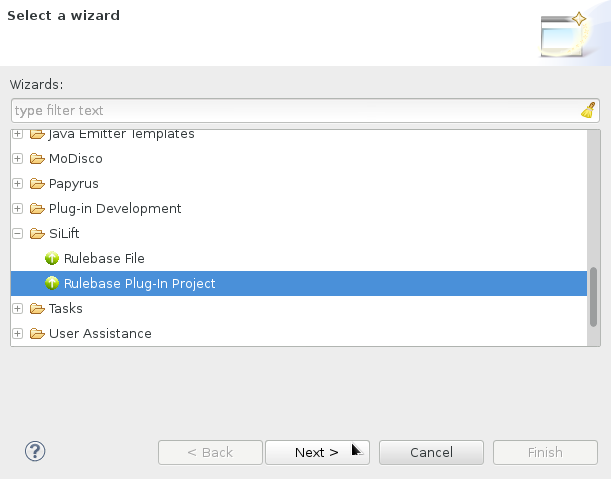
\includegraphics[width=0.6\textwidth]{recognitionrules/graphics/silift-wizard_rulebase_page01.png}
\caption{Erstellen eines \textit{Rulebase Plug-in Projects}}
\label{silift-wizard_rulebase_page01}
\end{figure}

Klicken Sie auf \texttt{Next} und geben Sie einen Projektnamen ein (vgl. Abb. \ref{silift-wizard_rulebase_page02}).

\begin{figure}[H]
\centering
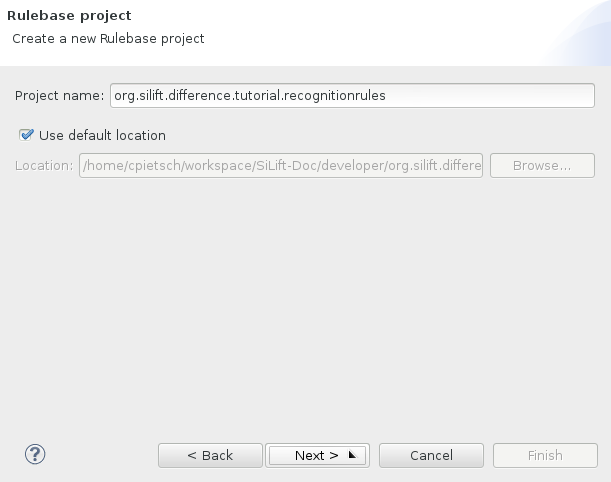
\includegraphics[width=0.6\textwidth]{recognitionrules/graphics/silift-wizard_rulebase_page02.png}
\caption{Erstellen eines \textit{Rulebase Plug-in Projects}}
\label{silift-wizard_rulebase_page02}
\end{figure}

Danach müssen noch die Editierregeln ausgewählt und unter einem entsprechenden Namen abgespeichert werden (vgl. Abb. \ref{silift-wizard_rulebase_page03}).
SiLift erzeugt nun die Erkennungsregeln und speichert diese in einer \textit{Rulebase}.

\begin{figure}[H]
\centering
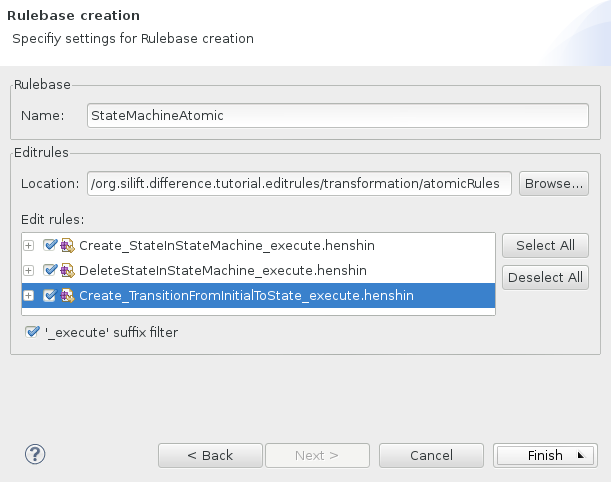
\includegraphics[width=0.6\textwidth]{recognitionrules/graphics/silift-wizard_rulebase_page03.png}
\caption{Erstellen eines \textit{Rulebase Plug-in Projects}}
\label{silift-wizard_rulebase_page03}
\end{figure}



\subsection{Rulebase File}
\label{sec:rbfile}

Des Weiteren kann es sein, dass Sie für eine Domain (hier unser Zustandsautomat) mehrere Regelbasen zur Verfügung stellen möchten.
Das ist z.B. dann der Fall, wenn man sich die Editierregeln mittels Generator hat generieren lassen und einige jetzt noch manuell nachgebessert oder ergänzt werden müssen.
Um eine neue Regelbasis zu erstellen, gehen Sie wieder auf \texttt{File} $\triangleright$ \texttt{New} $\triangleright$ \texttt{Other...} und wählen Sie  \texttt{SiLift} $\triangleright$ \texttt{Rulebase File}

\begin{figure}[H]
\centering
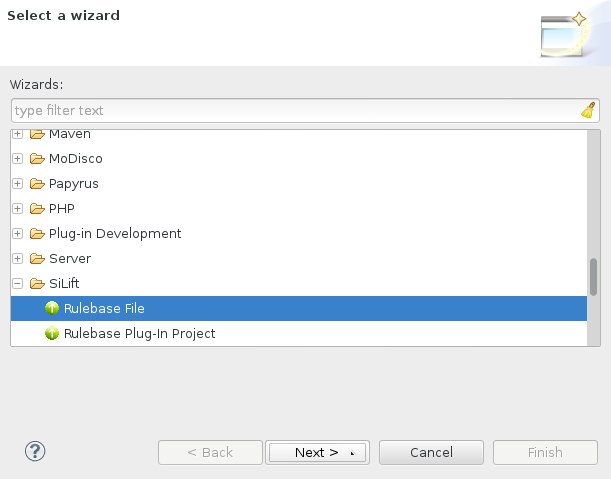
\includegraphics[width=0.6\textwidth]{recognitionrules/graphics/silift-wizard_rulebase_file_page01.png}
\caption{Erstellen einer neuen Regelbasis}
\label{silift-wizard_rulebase_file_page01}
\end{figure}

Im nächsten Schritt wählen Sie das Verzeichnis \texttt{rulebase} des bestehenden Projekts für die Erkennungsregeln und geben der Regelbasis einen Namen (vgl. Abb. \ref{silift-wizard_rulebase_file_page02}).

\begin{figure}[H]
\centering
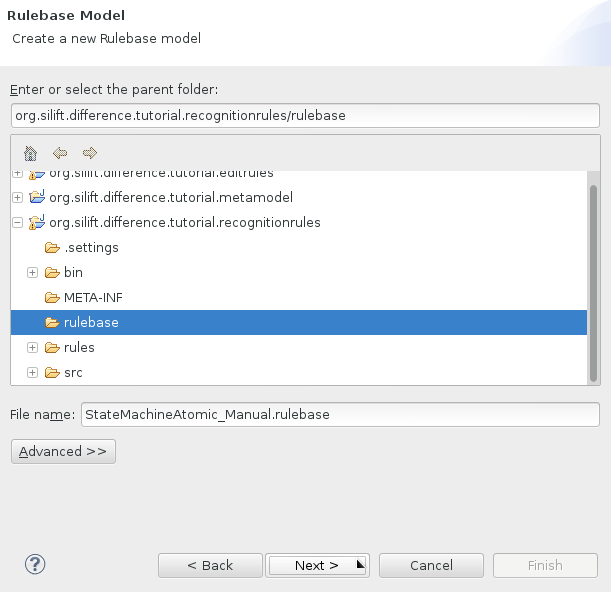
\includegraphics[width=0.6\textwidth]{recognitionrules/graphics/silift-wizard_rulebase_file_page02.png}
\caption{Erstellen einer neuen Regelbasis}
\label{silift-wizard_rulebase_file_page02}
\end{figure}

Jetzt wählen Sie wie bereits zuvor die gewünschten Editierregeln aus und klicken auf \texttt{Finish} (vgl. Abb. \ref{silift-wizard_rulebase_file_page03}).

\begin{figure}[H]
\centering
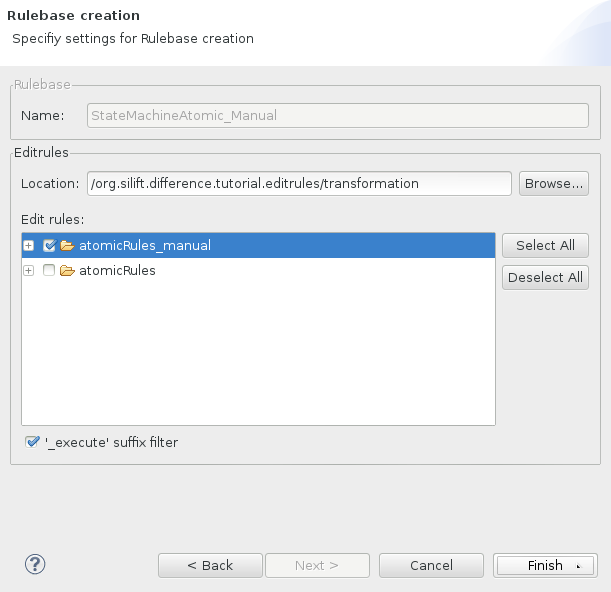
\includegraphics[width=0.6\textwidth]{recognitionrules/graphics/silift-wizard_rulebase_file_page03.png}
\caption{Erstellen einer neuen Regelbasis}
\label{silift-wizard_rulebase_file_page03}
\end{figure}

Damit haben Sie Ihrem Projekt eine neue Regelbasis hinzugefügt (vgl. Abb. \ref{silift-rulebase_package_explorer}).
Als nächstes muss sich diese Regelbasis noch als Erweiterung (engl. \textit{Extension}) bei dem Plugin registrieren.


\begin{figure}[H]
\centering
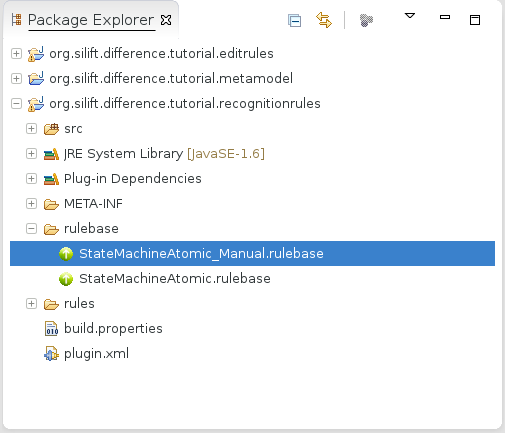
\includegraphics[width=0.3\textwidth]{recognitionrules/graphics/silift-rulebase_package_explorer.png}
\caption{Package Explorer: Regelbasen}
\label{silift-rulebase_package_explorer}
\end{figure}

Öffnen Sie das Verzeichnis \texttt{src} über den \textit{Package Explorer}, kopieren Sie die bereits existierende Klasse und nennen diese entsprechend um (vgl. Abb. \ref{silift-rulebase_class}).
Danach öffnen Sie die Klasse und passen den Wert der Variablen \texttt{RULE\_BASE\_NAME} entsprechend an. 

\begin{figure}[H]
\centering
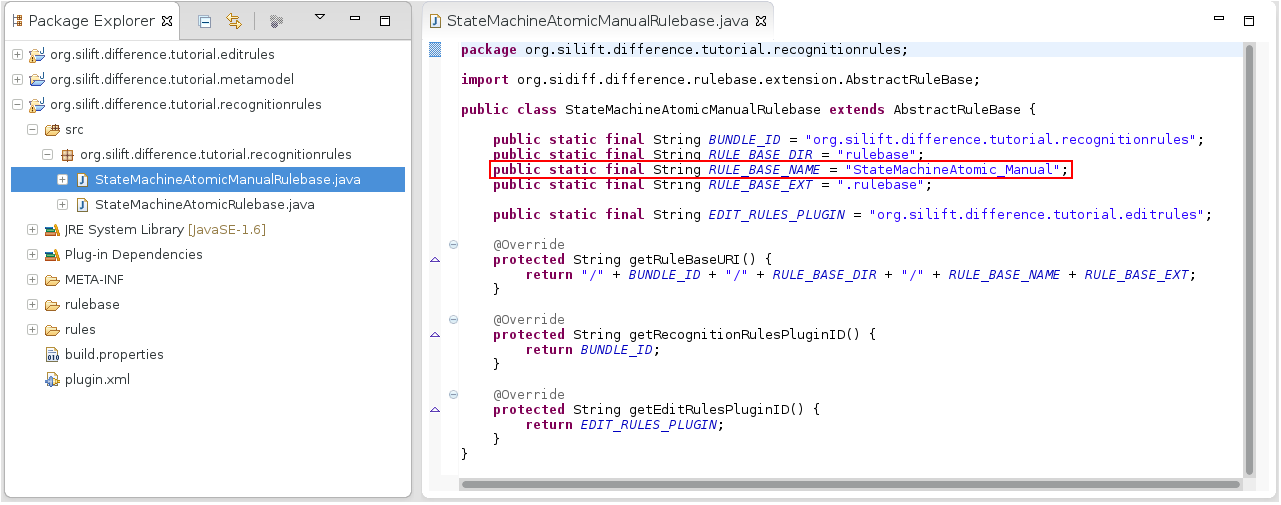
\includegraphics[width=0.8\textwidth]{recognitionrules/graphics/silift-rulebase_class.png}
\caption{Klasse: StateMachine\_AtomicManualRulebase}
\label{silift-rulebase_class}
\end{figure}

Öffnen Sie die \texttt{MANIFEST.MF} und wählen Sie den Reiter \texttt{Extensions} aus. 
Klicken Sie auf \texttt{Add...} und selektieren Sie den \textit{Extension Point} \texttt{org"".""sidiff"".""difference"".""rulebase"".""rulebase""\_extension}. Klicken Sie auf \texttt{Finish} (vgl. Abschnitt \ref{sec:own_matching_engine}).\\
Wechseln Sie danach in den Reiter \texttt{plugin.xml} und fügen Sie dem eben erstellen Extension Point die entsprechende URI der Erweiterung bei (vgl. Abb. \ref{silift-plugin_rulebase_manifest_plugin}).

\begin{figure}[H]
\centering
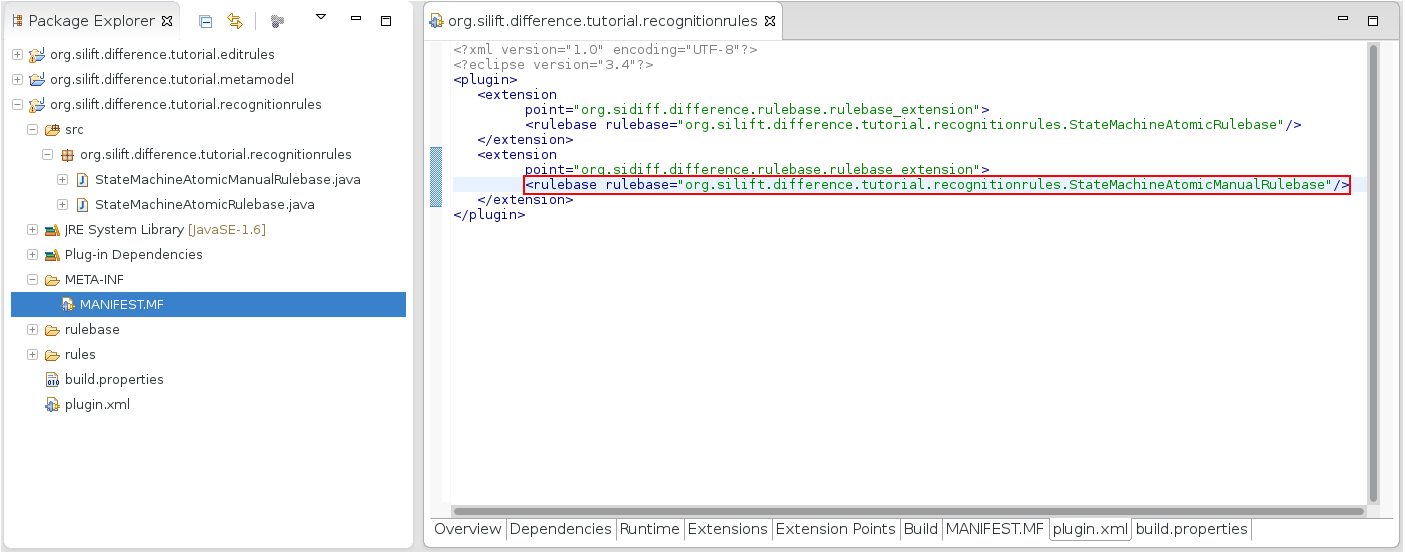
\includegraphics[width=0.8\textwidth]{recognitionrules/graphics/silift-plugin_rulebase_manifest_plugin.png}
\caption{Manifest.MF: \texttt{plugin.xml}}
\label{silift-plugin_rulebase_manifest_plugin}
\end{figure}



\subsection{Der Rulebase-Manager}
\label{sec:rbmanager}

Generierte Erkennungsregeln können mit Hilfe des \textit{Rulebase Manager} verwaltet werden (vgl. Abb. \ref{silif-rulebase_manager}).

\begin{figure}[H]
\centering
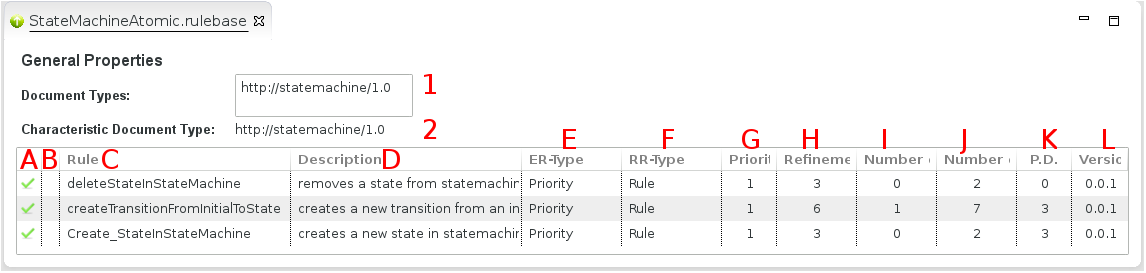
\includegraphics[width=0.8\textwidth]{recognitionrules/graphics/silift-rulebase_manager.png}
\caption{Erstellen eines \textit{Rulebase Manager}}
\label{silif-rulebase_manager}
\end{figure}

\begin{enumerate}
	\item Dokumenttypen der Regelbasis.
	\item Karakterisierender Dokumenttyp der Regelbasis.
\end{enumerate}

\begin{enumerate}[(A)]
\item Durch Klicken auf das Häkchen können einzelne Erkennungsregeln für die \textit{Recognition-Engine} aktiviert (grün) bzw. deaktiviert (grau) werden.

\item Zeigt an ob die zugehörige Editierregel valide ist. Sofern die Regel invalide ist wird ein Fehlersymbol angezeigt. Durch Klicken auf das Symbol wird der Validierungsfehler angezeigt.

\item Repräsentiert den Verwaltungsname der Editier-, bzw. Erkennungsregel. Dieser kann durch den Rulebase Manager editiert werden, wird aber nur zur Anzeige in der GUI verwendet.

\item Beschreibung der Editier-, bzw. Erkennungsregel.

\item Henshin Typ der \textit{mainUnit} der Editierregel (\texttt{Independent}, \texttt{Priority}, \texttt{Sequential} usw.).

\item Henshin Typ der Erkennungsregel (Rule und Multi-Rule).

\item Priorität der Erkennungsregel:
 Gerade unter zusätzlicher Verwendung komplexer Editierregeln kann es vorkommen, dass zwei Semantic Change Sets (vgl. \pageref{page:semantic_change_sets}) die gleichen low-level-Änderungen beinhalten. 
Für den Fall kann man einer Regel eine höhere Priorität zuordnen. 

\item \textit{Refinement-Level}: 
Für den Fall, dass auch die Prioritäten zweier identischer Semantic Change Sets gleich sind, versucht SiLift anhand der Anzahl der Supertypen die "'speziellere"' Regel zu bestimmen. 
D.h. je mehr Supertypen die Knoten der Regel besitzen, desto spezieller ist diese. 

\item Anzahl der positiven und negativen Application Conditions (PACs/NACs).

\item Anzahl der Parameter der Erkennungsregel.

\item \textit{Potential Dependicies}: 
Anzahl der potentiellen Abhängigkeiten zu anderen Editieroperationen. 
Das sequentielle Ausführen mehrere Editieroperationen ist nicht kommutativ, d.h. es können zwischen den jeweiligen Editieroperationen Abhängigkeiten existieren, die beim generieren eines Patches berücksichtigt werden müssen. 

\item Version der Erkennungsregel.
\end{enumerate}

I.d.R. wächst eine Regelbasis mit der Zeit. 
Es ist so gut wie unmöglich alle möglichen Editieroperationen im Vorfeld aufzudecken und zu implementieren. 
Um Ihrer bestehenden Regelbasis neue Regeln hinzuzufügen klicken Sie auf \texttt{Generate new recognition rules} (vgl. Abb. \ref{silift-rulebase_manager_create_new_rules}) und wählen die entsprechenden Editierregeln aus. 
Die abgeleiteten Erkennungsregeln werden nun der bestehenden Regelbasis hinzugefügt.

\begin{figure}[H]
\centering
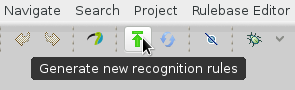
\includegraphics[width=0.25\textwidth]{recognitionrules/graphics/silift-rulebase_manager_create_new_rules.png}
\caption{Erkennungsregeln einer bestehenden \textit{Rulebase} hinzufügen}
\label{silift-rulebase_manager_create_new_rules}
\end{figure}


\subsection{Erkennungsregeln deployen und nutzen}
\label{sec:deploying_recognitionrules}

Um die Erkennungsregeln zu testen, gibt es zwei Möglichkeiten:

\begin{enumerate}

\item Eclipse Application: 
Öffnen Sie die \texttt{MANIFEST.MF} des Projekts der Erkennungsregeln und starten sie über das \textit{Launch Icon} (vgl. Abb. \ref{silift-rulebase_run_eclipse_application}) eine zweite Eclipse-Instanz. Innerhalb dieser Instanz sind alle Projekte aus Ihrem Workspace registriert und können verwendet werden.

\begin{figure}[H]
\centering
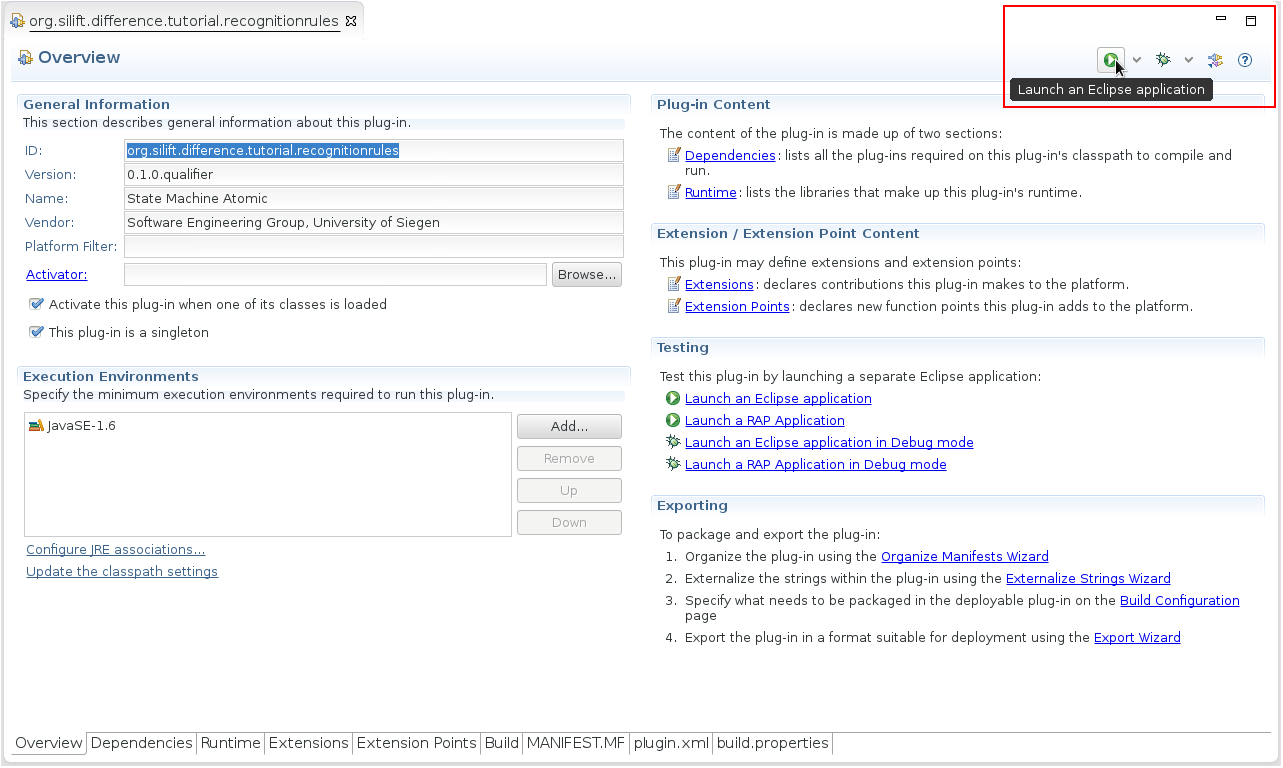
\includegraphics[width=0.8\textwidth]{recognitionrules/graphics/silift-rulebase_run_eclipse_application.png}
\caption{Run Ecplipse Application}
\label{silift-rulebase_run_eclipse_application}
\end{figure}


\item Deployable Plugins and Fragments: analog zu Abschnitt \ref{sec:own_matching_engine}.
\end{enumerate}

Wenn Sie Ihre Regeln erstmal nur testen möchten, ist die erste Variante zu bevorzugen. 
Sofern Sie die zweite Variante nutzen und ggf. mit Hilfe des \textit{Rulebase-Managers} an den Erkennungsregeln  etwas verändern möchten, müssen Sie die installierten Plugins zuerst deinstallieren.\\

Eine umfassende Einführung in die Nutzung von SiLift als Differenzwerkzeug finden Sie im \textbf{SiLift - Benutzerhandbuch für Endanwender}.